\subsection{Overview}
DREAM will be used by thousands of users each day, with different needs, and located all over the Telangana region.\\
To achieve this result and to respect all the requirements stated in the RASD, DREAM will be developed as a distributed application with clients and servers.\\
The client will only show the graphical interface to the end-user, while the back-end will execute and support all the business logic operations. 
\begin{figure}[hbt!]
\centering
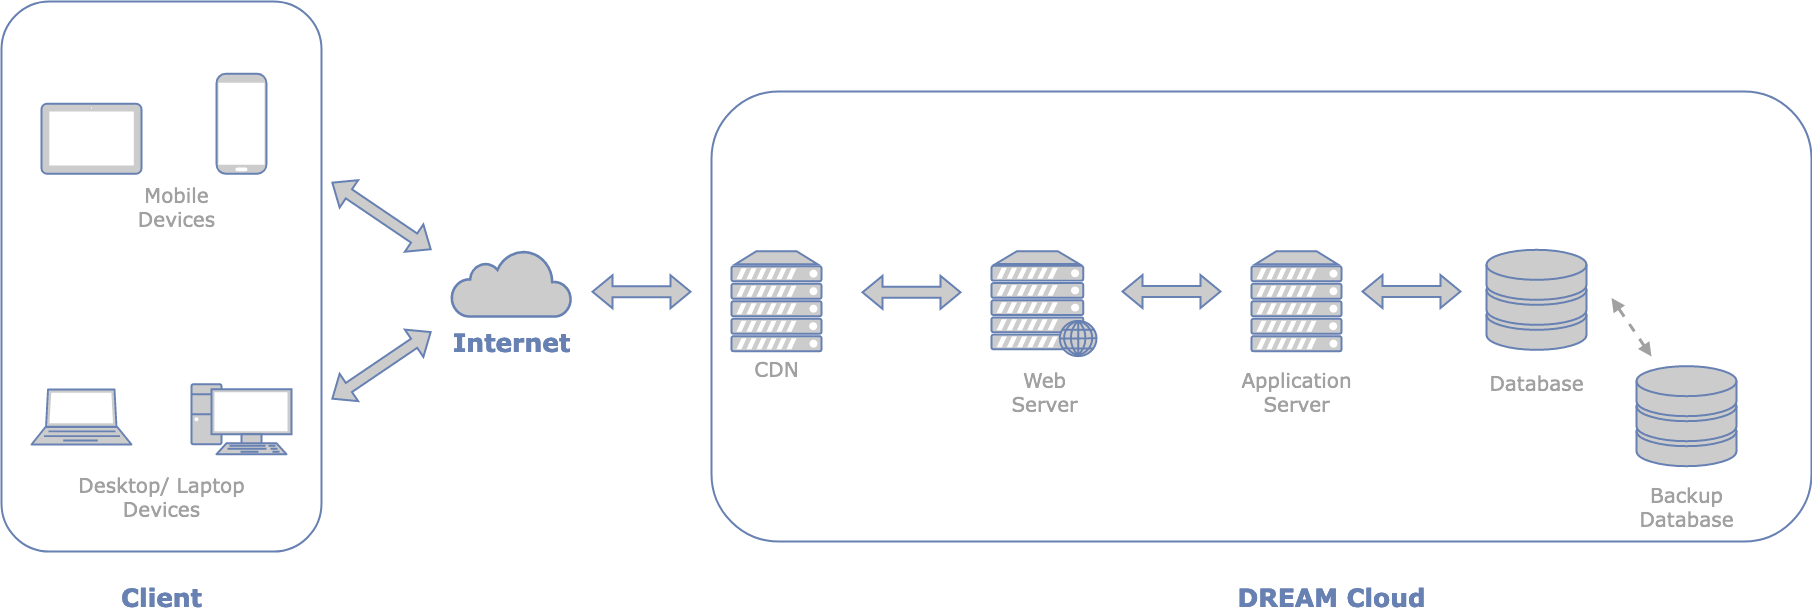
\includegraphics[width=\textwidth]{../images_diagrams/dd/highlevel_arch.png}
\caption{High-Level 5-tier Architecture.}
\label{fig:highLevelArch}
\end{figure}

Since the application must be reliable and flexible enough in handling the growth of the user base, a cloud-based architecture seems to be suited for this task.\\
In particular, DREAM Cloud is a 3-tier architecture with a WebServer, an Application Server, and a Storage Server (DBMS Server).\\
To allow the system to work always in ideal conditions, a load balancer routes all the requests to different application servers: if necessary, new instances of the servers should be created and used to balance the computational load.\\
An additional tier is then placed between the user and the DREAM Cloud: a Content Delivery Network (CDN) will relieve some load from the system and improve performances in serving static contents. Overall, the resulting application will have five tiers.\\
Lastly, given the importance of the historical data kept inside the database, a backup system clone frequently the data on a different server, possibly located in a different availability zone.\\ 

\subsection{Component View}

\begin{figure}[hbt!]
\centering
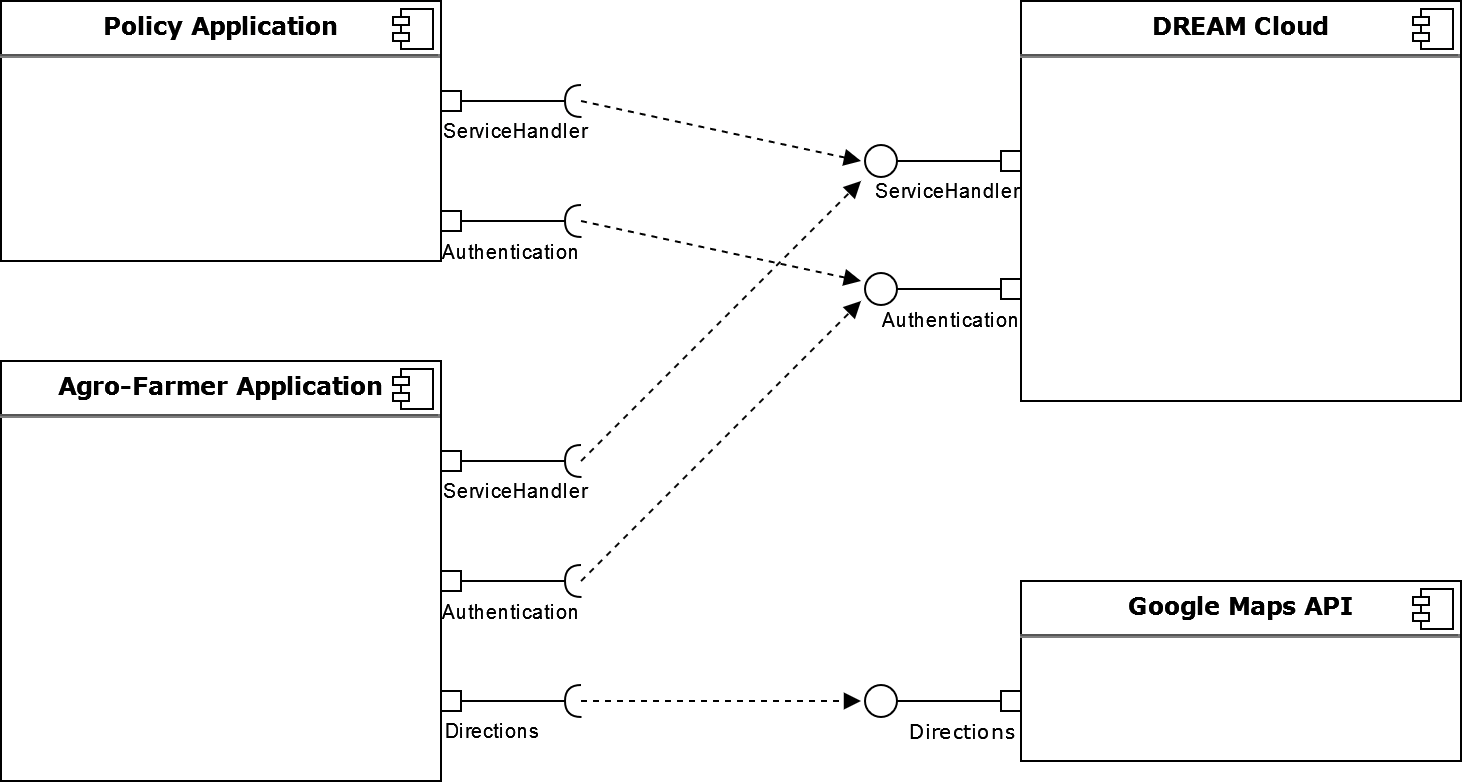
\includegraphics[width=\textwidth]{../images_diagrams/dd/high_level_cloud.png}
\caption{High-Level Component View.}
\label{fig:highLevelComp}
\end{figure}

\subsection{Deployment View}
\begin{figure}[hbt!]
\centering
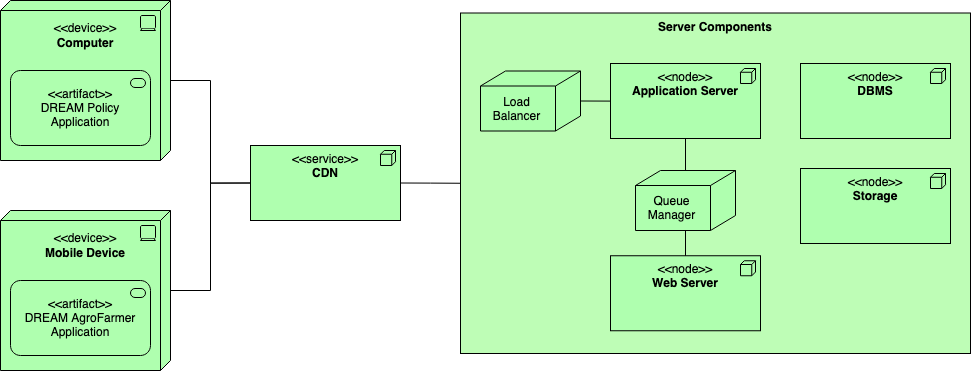
\includegraphics[width=\textwidth]{../images_diagrams/dd/highlevel_deployment.png}
\caption{High-Level Deployment View.}
\label{fig:highLevelDeploy}
\end{figure}

\begin{flushleft}
The main components in the deployment view in Figure \ref{fig:highLevelDeploy} are the client devices and the cloud platform. Policy makers will access the DREAM Policy Application via a computer device whereas agronomists and farmers will access the DREAM AgroFarmer Application via a mobile device. The CDN is represented as an external service. Then, the server components of the DREAM cloud include the application server, the web server, the database server, and the storage server. Within the cloud platform there is also a load balancer and a queue manager.
\end{flushleft}




\subsection{Runtime View}
You can use sequence diagrams to describe the way components interact
to accomplish specific tasks typically related to your use cases
\subsection{Component Interfaces}
\subsection{Selected Architectural Styles and Patterns}
Please explain which styles/patterns you used, why, and how
\subsection{Other Design Decisions}